\chapter{The OSM Extractor Extension}\label{ch:the-osm-extractor-extension}
\section{Overview}
The \textbf{OSM Extractor} extension is an extension build using the OpenRefine extension architecture and its purpose
is to integrate OpenStreetMap data into a new OpenRefine project.
The OpenStreetMap data is retrieved by sending an Overpass QL query to the Overpass API which then
returns the OSM data as XML as response.
This data then goes through a conversion process which converts the OSM data to Simple Feature geometries.
\section{OpenStreetMap and the Overpass API}
OpenStreetMap is a free map of the world in which people around the world continuously contribute to.
The map is freely accessible on the web and any change that is made is automatically owned by the user who changed it.
The Overpass API is a read-only API which users can use to select custom parts of OSM data.
The client sends a query to the API and the API returns the OSM data selected by the query.
\subsection{OpenStreetMap data (Elements)}
Elements (or objects) are the basic components of OpenStreetMap's conceptual data model of the physical world. They consist of:
\begin{itemize}
    \item Nodes (defining points in space)
    \item Ways (defining linear features and area boundaries)
    \item Relations (which are sometimes used to explain how other elements work together).
\end{itemize}
All of the above can have one or more associated tags (which describe the properties (usually non-spatial) of a particular element). \cite{OSMElements}
Tags have a [key=value] format and they describe features of map elements.
There is no restrictions on the format of the tags but every type of element should have their own "standardized" tags which
are usually used to display such features.
An example of this would be that restaurant tags (amenity=restaurant) are usually used
in combination with other tags such as [name=*], [cuisine=*] etc.\\
\newline
More information on OpenStreetMap tags and their popularity can be found under \href{https://taginfo.openstreetmap.org/}{https://taginfo.openstreetmap.org/}\\
\newline
Example of an OSM node (including its metadata), represented using the official OSM data representation (XML):
\begin{minted}[tabsize=2,breaklines, linenos]{xml}
 <node id="1831881213" version="1" changeset="12370172" lat="54.0900666" lon="12.2539381" user="lafkor" uid="75625" visible="true" timestamp="2012-07-20T09:43:19Z">
  <tag k="name" v="Neu Broderstorf"/>
  <tag k="traffic_sign" v="city_limit"/>
 </node>
\end{minted}
\subsection{The Overpass API}
OpenStreetMap data can be queried over the web with the help of the \href{https://wiki.openstreetmap.org/wiki/Overpass_API}{Overpass API}.
The Overpass API keeps a copy of the main database up to date with these minute updates and provides them for search.
There exist not only public instances to which a request can be sent.
It is also possible to have your own instance because Overpass API is open source
with easy installation and reasonable hardware requirements. \cite{WhatIsOverpassAPI}\\
\newline
\href{https://overpass-turbo.eu/}{The Overpass Turbo} web application can be used to quickly visualize any query made to the Overpass API.
It provides the user with an editor for writing the query to send to Overpass and as soon as the query is processed and the data is returned,
it immediately gets displayed on a map.\\
\newline
\subsubsection{Overpass QL}
The Overpass API accepts two types of query languages: \href{https://wiki.openstreetmap.org/wiki/Overpass_API/Language_Guide#The_Overpass_API_languages}{Overpass XML}
and \href{https://wiki.openstreetmap.org/wiki/Overpass_API/Overpass_QL}{Overpass QL}.
In this project, the Overpass QL (the second query language created for the Overpass API) is used to query OpenStreetMap data.
It is a procedural, imperative programming language written with a C style syntax. \cite{WhatIsOverpassQL}\\
\newline
Here's an example of an Overpass QL query, which queries bus stops with shelter and inside a specific bounding box:\\
\begin{minted}[tabsize=2,breaklines, linenos]{sql}
node
  ["highway"="bus_stop"]
  ["shelter"="yes"]
  (50.7,7.1,50.8,7.25);
out body;
\end{minted}
\pagebreak
\section{Implementation}
\subsection{Overview}
The extension adds a new import option in OpenRefine called \textit{OpenStreetMap (Overpass)} which allows the user to choose a
public Overpass API instance on the web and enter an Overpass QL query inside the text area.\\
\newline
The public API instances offered by the extensions are:
\begin{itemize}
    \item \href{https://lz4.overpass-api.de/api/interpreter}{https://lz4.overpass-api.de/api/interpreter}
    \item \href{https://z.overpass-api.de/api/interpreter}{https://z.overpass-api.de/api/interpreter}
    \item \href{https://overpass.openstreetmap.ru/api/interpreter}{https://overpass.openstreetmap.ru/api/interpreter}
    \item \href{https://overpass.openstreetmap.fr/api/interpreter}{https://overpass.openstreetmap.fr/api/interpreter}
    \item \href{https://overpass.osm.ch/api/interpreter}{https://overpass.osm.ch/api/interpreter}
    \item \href{https://overpass.kumi.systems/api/interpreter}{https://overpass.kumi.systems/api/interpreter}
    \item \href{https://overpass.nchc.org.tw/api/interpreter}{https://overpass.nchc.org.tw/api/interpreter}
\end{itemize}
The Overpass QL is wiped out of comments before processing and has the following restrictions:
\begin{itemize}
    \item \mintinline{sql}{[out:json]} is not allowed
    \item \mintinline{sql}{[out:csv]} is not allowed
    \item \mintinline{sql}{out center;} is not supported, more information on why it is not supported can be found
    on the design decisions of the extension above
\end{itemize}
\begin{figure}[H]
    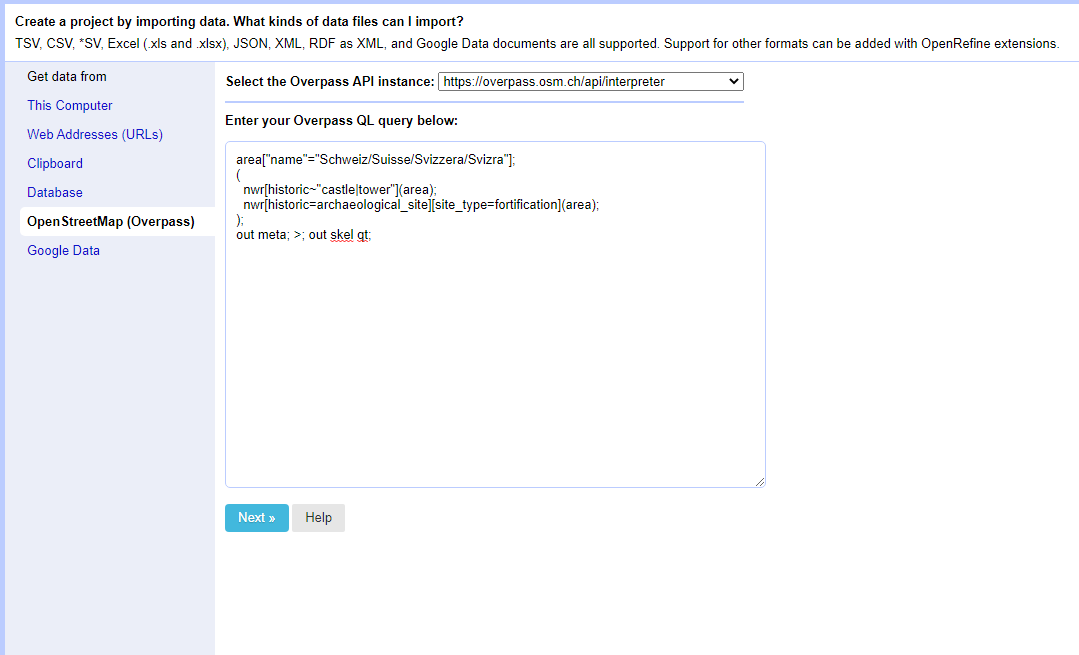
\includegraphics[width=\linewidth]{./Figures/OSM_Extractor/osm_extractor_import_page.png}
    \caption{The \textit{OpenStreetMap (Overpass)} import option in OpenRefine}
\end{figure}
After the user enters a valid Overpass QL query and selects the Overpass API instance, a request is made to that API instance and
the user is presented with a new page where they can configure the mapping options for the OpenStreetMap data. More information on
this step is explained more thoroughly in this
\hyperref[sec:mapping-preparation-of-openstreetmap-data]{chapter}.
\subsection{Mapping \& Preparation of the OpenStreetMap Data}\label{sec:mapping-preparation-of-openstreetmap-data}
When the user hits on the \textit{Next} button, a new page is shown with a loading screen where the user has to wait until
the request is finished (with success or not). Some Overpass QL queries can take a long time to proceed and that's why
the user can abort the query anytime using the\textit{Abort} button below the loading icon. If they abort the request,
the user is sent back to the import (index) page of OpenRefine.\\
\newline
After the query finishes processing, the OpenStreetMap XML data is then stored in memory and ready to be processed and
imported into a new project (made possible by the osm4j library).
\newline
When all the above tasks are finished, the user is presented with a table of tags and some parsing options below where they
can select what types of Geometry they want to include in the project and also some other settings. The table contains
all the available tags from all the OSM elements, metadata tags and also identifier tags. \\
\newline
The user can override the new column name to be different than from the tag name by changing the value on the
\textit{Column name} column of the table. They can also completely exclude/include a tag (or rather a column now) from being created
by selecting/de-selecting the checkbox in the beginning of the row. Some of the OSM tags are considered as \textbf{Main}
tags while the others are considered as \textbf{Other} tags. These can be viewed on the \textit{Type} column of the table.\\
\newline
\textbf{Main} tags are all the tags that define real-world objects and not properties of such.
A tag is considered as important or as a \textbf{Main} tag if it belongs to the following list:
\textit{aerialway, aeroway, amenity, barrier, boundary, building, craft, emergency, ford, geological, highway, historic,
landuse, leisure, man\_made, military, natural,
office, place, power, public\_transport, railway, shop, tourism, waterway, type, entrance, pipeline, healthcare,
playground, attraction, traffic\_sign, traffic\_sign:forward, traffic\_sign:backward, golf, indoor, cemetry, building:part,
landcover, advertising, traffic\_calming, club, cemetery, police, telecom.}\\
\newline
This list of "main" tags has been taken from \href{https://github.com/simonpoole}{Simon Poole's} \textit{OSM preset utils}
repository \href{https://github.com/simonpoole/preset-utils/blob/master/src/main/java/ch/poole/osm/presetutils/Tags.java}{here}.\\
\newline
\textbf{Identifier}, \textbf{Meta} and \textbf{Main} tags are automatically selected by the extension, other tags can 
be included in the project by selecting the checkbow on the appropriate row.
\begin{figure}[H]
    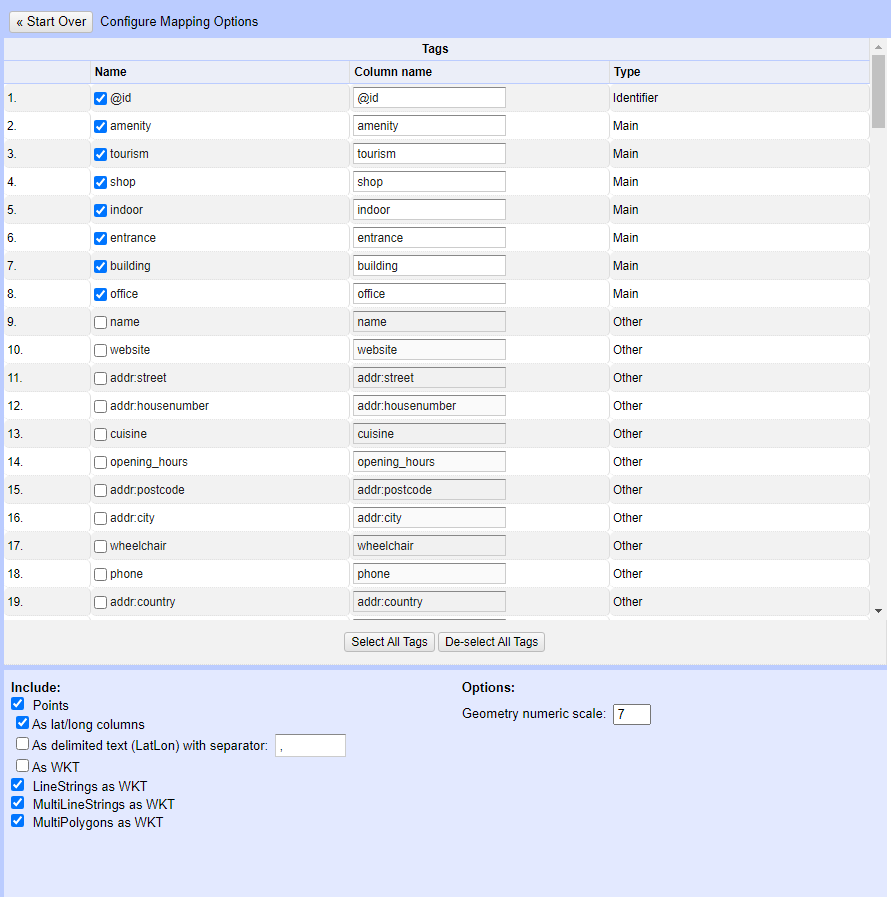
\includegraphics[width=\linewidth]{./Figures/OSM_Extractor/osm_extractor_parsing_table.png}
    \caption{The \textit{OpenStreetMap (Overpass)} mapping \& parsing options in OpenRefine}
\end{figure}
Below the table, there are also options on what types of geometries to include in the project and also some other extra options.
Users can include:
\begin{itemize}
    \item Points
        \subitem As lat/long columns
        \subitem As lat/long delimited column e.g. \textit{47.4955184, 8.741556}
        \subitem As WKT
    \item LineStrings as WKT
    \item MultiLineStrings as WKT
    \item MultiPolygons as WKT
\end{itemize}
These types of geometries are \textit{Simple Feature} geometries and the OSM elements are converted to such
features during the conversion phase. These concepts and this process is thouroughly described in the
\hyperref[sec:conversion-to-simple-features-geometry]{Conversion to Simple Features Geometry} chapter.\\
\newline
The user can also select the numeric scale of the decimal values of the geometries by tweaking the \textbf{Geometry numeric scale}
option to a different number, the default value is \textbf{7}. This number represents the number of decimal digits to the right
of the decimal point of a decimal number, e.g. \textit{47.4955184} has a numeric scale of 7 because there are 7 numbers to
the right of the decimal point of the number (this being the default numeric scale). This numeric scale is used
while processing lat/lon values or WKT values. \\
\newline
More information on what a numeric scale is can be found here:
\href{https://docs.microsoft.com/en-us/sql/t-sql/data-types/precision-scale-and-length-transact-sql?view=sql-server-ver15}{https://docs.microsoft.com/en-us/sql/t-sql/data-types/precision-scale-and-length-transact-sql?view=sql-server-ver15}.
\subsubsection{Conversion to Simple Features Geometry}\label{sec:conversion-to-simple-features-geometry}
When the OpenStreetMap XML data is received, it is received as nodes, ways and relations. This extension however, converts such
elements to \href{https://www.ogc.org/standards/sfa}{Simple Feature Geometry} before inserting it into OpenRefine.\\
\newline
In the parsing options, at the bottom, there exist the types of Geometries to include in the project, they are all part of the \textit{Simple Feature} geometry objects:
\begin{itemize}
    \item Points (as lat/lon, as delimited text and as WKT)
    \item LineStrings as WKT
    \item MultiLineStrings and
    \item MultiPolygons
\end{itemize}
To convert such data into \textit{Simple Feature} geometry, a combination of the \href{https://github.com/topobyte/osm4j}{osm4j}
(it has some geometry and utility functions essential for the conversion) and
\href{https://github.com/locationtech/jts}{JTS Topology Suite} (for providing \textit{Simple Feature} geometry classes and functions) library is used.\\
\newline
Here's the Java code that e.g. does the conversion of an OSM node to a JTS \mintinline{bash}{Point} Geometry:
\begin{minted}[breaklines, linenos, tabsize=2]{java}
    NodeBuilder nodeBuilder = new NodeBuilder();
    osmExtractor.addPoint(nodeBuilder.build(node), node.getId(), OsmModelUtil.getTagsAsMap(node), node.getMetadata());
\end{minted}
This portion of code uses osm4j\textquotesingle s NodeBuilder class to build a JTS Point Geometry. Other parameters are necessary attributes for the Point such as:
the identifier, its OSM tags and its metadata.\\
\newline
Creating \mintinline{bash}{LineStrings}, \mintinline{bash}{MultiLineStrings} and \mintinline{bash}{MultiPolygons} is not
as straightforward as creating \mintinline{bash}{Points}, hence a combination of methods is used to make such a conversion possible.
The library of osm4j handles a lot of the logic of those conversions (geometry functions) while the JTS library stores
them in their appropriate Java classes as Geometry objects. Other Java classes provided by this extension bundle up the JTS geometries along
with their OSM attributes in a single object. This makes it easy for storing the whole OSM element (and its attributes)
along with its \textit{Simple Feature} geometry attributes.
\subsection{Creating the Project in OpenRefine}
After all the desired tags have been selected and the geometries have been included, the user can choose a
name for the newOpenRefine project and select the \textit{Create Project} button at the top right of the
page in order to initiate the creation of a new OpenRefine project.
The creation process is executed on a separate thread and utilizes OpenRefine's core engine to do so.
The process shouldn't take very long before it's fully completed.
\subsubsection{The Project}
The created project has columns of the tags that were selected in the mapping \& parsing stage. There will be some extra columns,
depending on what options were selected. For example, if points were included as lat/long, there will be two columns called \textit{latitude}
and \textit{longitude} that contain the value of X and Y of the points. Moreover, if the \textit{Points as delimited text} option was selected,
another column called \textit{point\_delimited} is added containing latitude/longitude columns, separated with
the selected separator in the mapping options. Finally, there will be the \textit{WKT} column which contains
the WKT string for the geometry. All of the values of these extra columns (latitude, longitude, WKT) have the precision scale of the one that was entered in
the mapping options. The project\textquotesingle s description also consists of the Overpass QL query that was entered initially.\\
\newline
Some of the values have a green color instead of the native black one, this means that the data type of those values is other
than text i.e.\ number, date or boolean.
OpenRefine treats data types differently from one another and all of the data types
have their own functions (apart from the inherited ones) which can be performed
only on them.\\
\begin{figure}[H]
    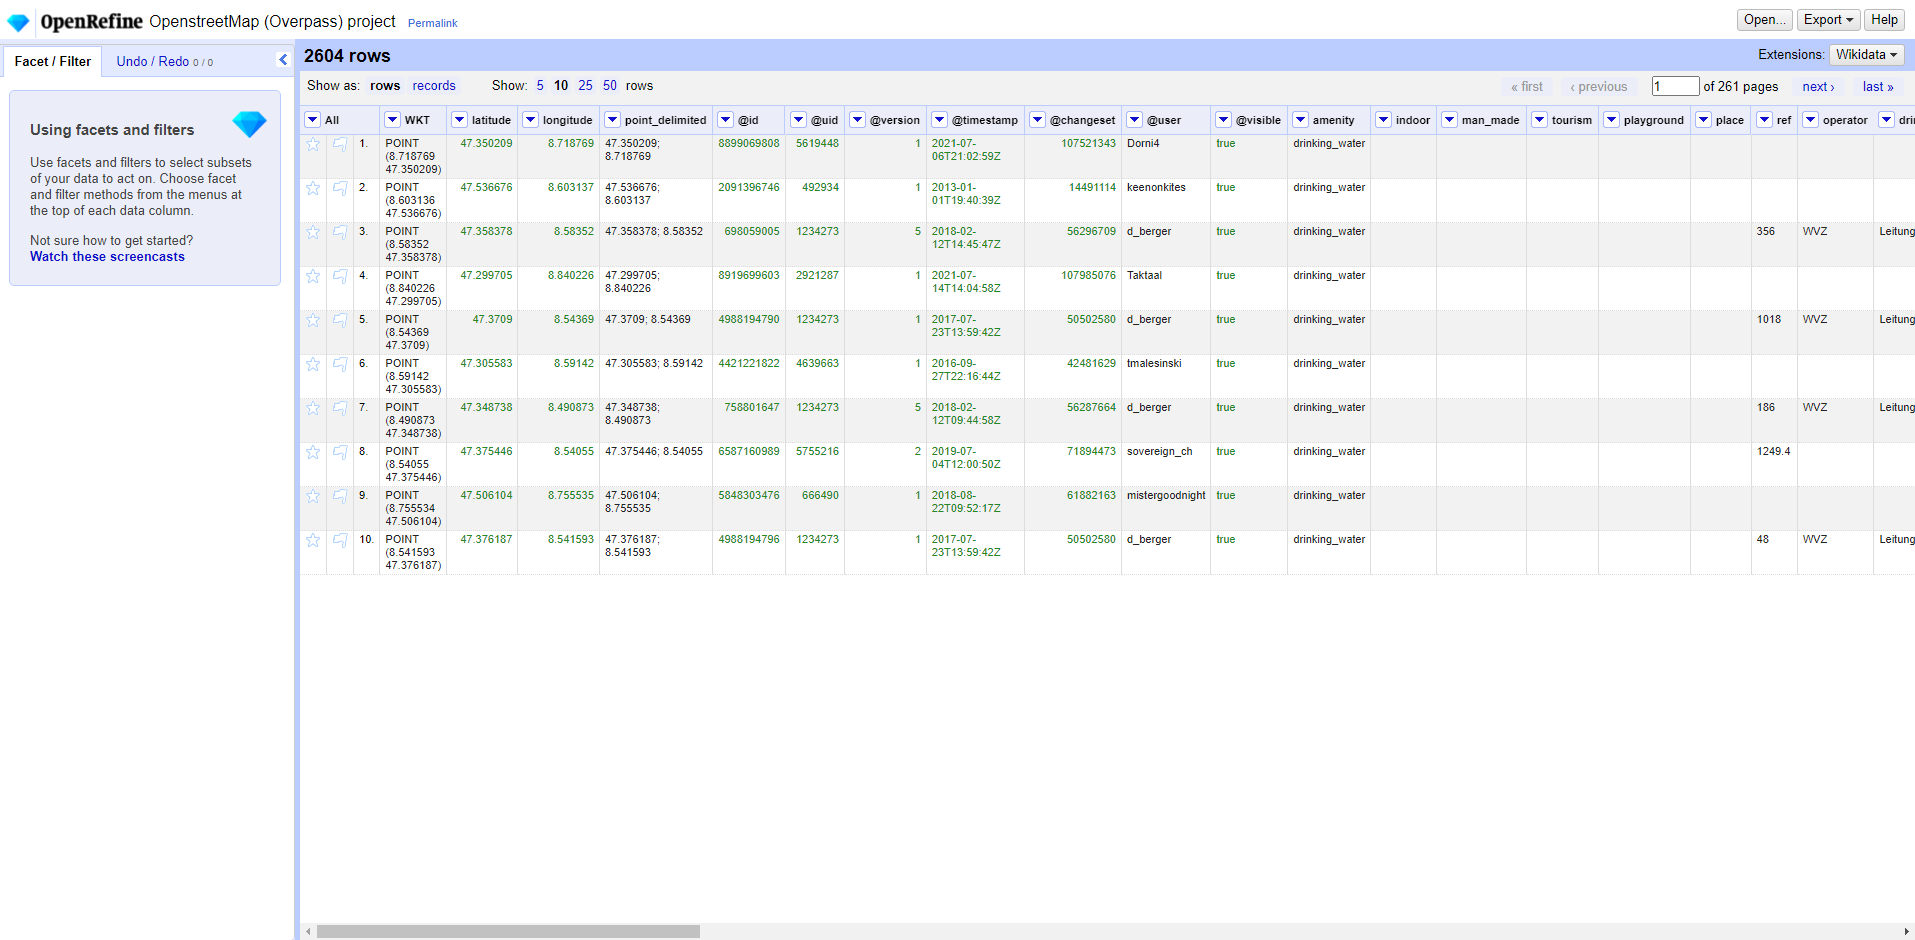
\includegraphics[width=\linewidth]{./Figures/OSM_Extractor/osm_extractor_project.png}
    \caption{An OpenRefine project, created using the OSM Extractor extension}
\end{figure}
\subsection{The \mintinline{java}{interiorPoint()} function}
The OSM Extractor extension also includes a new GREL function called \mintinline{java}{interiorPoint()}. This function
utilizes the \href{https://github.com/locationtech/jts}{JTS} library in order to compute the interior point of a Geometry.\\
\newline
OpenRefine offers interfaces which allow the developer to add new GREL functions to the project. Such interfaces were used in order
to add this GREL function. The \mintinline{java}{interiorPoint()} function takes one argument: a WKT string containing the geometry
of which the user wants to compute the interior point of and returns a WKT containing a Point Geometry of the computed interior point.\\
\newline

Here's the GREL function and how it computes the interior point of a Geometry:
\begin{minted}[tabsize=2, breaklines, linenos]{java}
    Geometry geometry = new WKTReader().read((String) args[0]);
    Point point = org.locationtech.jts.algorithm.InteriorPoint.getInteriorPoint(geometry);
    return new WKTWriter().writeFormatted(point);
\end{minted}
The first line reads the argument that was provided by the user as WKT and converts it to JTS Geometry.
The second line utilizes JTS's \mintinline{java}{getInteriorPoint()} function to compute the interior point of the
given geometry. The results are then returned back to the user as a WKT string.\\
\newline
This function is useful for Wikidata reconciliation with OpenStreetMap elements (available in OpenRefine).
This converts OSM Polygons (or any type of Geometry) to Points (with coordinates) since Wikidata only knows coordinates.
\pagebreak
\subsection{Testing}
This extension includes some unit testing. The framework used for unit testing is the \href{https://testng.org/}{TestNG} framework.
\subsection{Unit Testing}
TestNG is a testing framework inspired from JUnit and NUnit. It is designed to cover all categories of testing.\\
\newline
This extension contains minimal unit testing for some of its important functions and everytime the CI/CD pipeline is run in GitLab, the
extension's unit tests are executed to see if everything is still working as expected.
\pagebreak
\section{Usage \& Examples}
\subsection{Usage}
\begin{enumerate}
    \item Launch OpenRefine with the \textbf{OSM Extractor} extension
    \item In the index page, choose \textit{OpenStreetMap (Overpass)} from the import options
    \item Choose another Overpass instance or leave the default one in the select list
    \item Enter an Overpass QL query inside the text area
        \subitem Make sure you test the query inside \href{https://overpass-turbo.eu/}{Overpass Turbo} to get a clearer
        picture of the data before using it in the extension.
    \item Click on the \textit{Next} button and wait for the query to be finished (It can be aborted anytime by clicking on the \textit{Abort} button)
    \item Choose the tags you want to include in the OpenRefine project and override the column names for each tag if necessary
    \item Choose the geometries to include, some of them are automatically selected
    \item Override the \textit{Geometry numeric scale} if necessary, choose a project name and click on the \textit{Create Project} button
\end{enumerate}
\subsection{Examples}
Here are some Overpass QL examples that were highly used while developing \& testing this extension:
\begin{minted}[tabsize=2, breaklines, linenos]{sql}
area["name"="Prishtinë"];
(
  nwr[amenity="cafe"](area);
);
out body;
\end{minted}
This \href{https://overpass-turbo.eu/s/1aTT}{query} returns all the cafe bars in Prishtina, Kosovo.
It returns only points as no recurse function was used to produce the full result set.
\begin{minted}[tabsize=2, breaklines, linenos]{sql}
area["name"="Schweiz/Suisse/Svizzera/Svizra"];
(
  nwr[historic~"castle|tower"](area);
  nwr[historic=archaeological_site][site_type=fortification](area);
);
out meta; >; out skel qt;
\end{minted}
This \href{https://overpass-turbo.eu/s/1aTT}{query} returns all the castles of Switzerland, including their OSM metadata.
\begin{minted}[tabsize=2, breaklines, linenos]{sql}
area["name"="Los Angeles"];
(
  nwr[amenity=restaurant](area);
);
out body; >; out skel qt;
\end{minted}
This \href{https://overpass-turbo.eu/s/1aTR}{query} returns all the restaurants in Los Angeles, California, without the OSM metadata.
\begin{minted}[tabsize=2, breaklines, linenos]{sql}
area["name"="Chur"];
(
  nwr[highway=residential](area);
)
(._;>;);
out body;
\end{minted}
This \href{https://overpass-turbo.eu/s/1aTV}{query} returns all the residential highways (or streets used for local traffic) inside Chur, Switzerland.